\documentclass[11pt]{article}    

\usepackage{writeup}

\title{Greed is Feed: An Attempt to Find a Fair Selection Scheme Amidst Inequality}
\author{Nicholas Pun}

\begin{document}
\maketitle

\vspace{3mm}
\begin{center}
    \parbox{0.85\textwidth}{%
    \it{Abstract.}
    Suppose $m$ players select from a pool $\U$ of $n$ elements without replacement and with the additional restriction that their selections are limited to subsets $\U_1, \ldots, \U_m \subseteq \U$, respectively.
    When the $U_i$'s only partially intersect, a prior player's selection may not affect all the players coming after them.
    Further, by changing the order that the $m$ players draw from the pool, we may increase or decrease the probability of an element being chosen once it reaches a later player.
    What ordering will yield the most uniform probabilities for every player?
    In this paper, we answer this for the $2$-player case and show that being ``greedy'' in our ordering may not yield optimal results for a very specific instance of a $10$-person case through empirical results.}
\end{center}
\vspace{5mm}

{\small \tableofcontents}

\section{Motivation}\label{Section:Motivation}

The idea for this problem came from the All Random, All Mid (ARAM) game mode in popular multiplayer online game \it{League of Legends}\footnote{https://na.leagueoflegends.com/en-us/}.
In this game mode, two teams of $5$ are randomly given characters (known as champions) to battle against each other and take out the opponent's home base first.
There are several rules in play when players randomly select their champions:
\begin{itemize}
    \item There is a universal pool of $152$ champions\footnote{As of October 29th, 2020} to select from and selections occur without replacement 
    \item Players don't immediately have access to the entire pool and must purchase additional champions to increase their personal pool. This will result in different players having access to different subsets of the universal pool.
    \item There are always 14 champions that are \it{``free-to-play''} or accessible to all $10$ players. (This prevents the case where a player runs out of champions to select from their pool)
    \item Players line-up in some order to make their selections
\end{itemize}
The last rule makes for an interesting probabilistic concern since a prior player's selection may only affect a fraction of the players after them (since some players may not have access to that champion in their personal pool).
This differs from the case where everyone has access to the universal pool and are uniformly affected by a prior player's selection.
As such, we might expect that as we change the ordering of the players, their individual probabilities of selecting a particular champion will change as well.

To see this concretely, let's consider the scenario where there are only 2 players.
Player A has access to only 2 champions from the universal pool while Player B has access to the entire universal pool.
If Player A goes first, regardless of the champion that is selected, Player B will have less champions to choose from.
However, if Player B goes first, there is a probability that they select a champion that is inaccessible to Player A.
As such, Player A's pool will be unaffected when it comes to their turn to choose.
We will delve more into this example in \Cref{Section:Two-Player}.

\section{Problem Definition}\label{Sec:Problem-Definition}

In this section, we will present a generalization of the problem described in \Cref{Section:Motivation} and also refine the questions we want to answer in this paper.

Let $\U = \{u_1, \ldots, u_n\}$ be the universal pool of $n$ elements and $\U_1, \ldots \U_m \subseteq \U$ be the individual pools for Players $P_1$ through $P_m$ respectively.
Let $\sigma: [m] \longrightarrow [m]$ be an ordering of the $m$ players.
(So, $P_{\sigma(1)}$ is the player that goes first, $P_{\sigma(2)}$ second and so forth)
Suppose the $m$ players pick from $\U$ using the following scheme:

\IncMargin{2em}
\begin{algorithm}[H]
    \SetKwInOut{Input}{Input}\SetKwInOut{Output}{Output}
    
    \BlankLine
    \Input{Universal pool $\U$, player pools $\U_1, \ldots, \U$, and player ordering $\sigma$}
    \Output{An assignment of $P_1, \ldots, P_m$ to unique elements $u_{P_1}, \ldots, u_{P_m}$}
    \BlankLine

    $\U_{\mathtt{curr}} \leftarrow \U$

    \For{$i \leftarrow 1$ \KwTo $m$}{
        Select an element $u_j$ (uniformly at random) from $\U_{P_{\sigma(i)}} - \U_{\mathtt{curr}}$ and assign it to $P_{\sigma(i)}$
        
        $\U_{\mathtt{curr}} \leftarrow \U_{\mathtt{curr}} - \{u_j\}$
    }
\end{algorithm}
\DecMargin{2em}

We've already seen that changing the order of the players has an impact on the individual probability distributions.
(We will also show this more carefully in \Cref{Section:Mathematical-Approach})
Since we're ultimately playing a game, it's natural to want an ordering that maximizes fairness.
That is, we want an ordering of players such that the probability for player $P_i$ to select element $u \in \U_i$ is \it{close to} uniform $\left(\frac{1}{|\U_i|}\right)$.
By \it{close to}, we mean that the following metric should be minimized:

\begin{definition}[Hellinger Distance\footnote{See \url{http://encyclopediaofmath.org/index.php?title=Hellinger_distance&oldid=47206}}]
    Let $P = (p_1, \ldots, p_k)$, $Q = (q_1, \ldots, q_k)$ be two discrete probability distributions, their \it{Hellinger distance} is defined as:
    \[
        H(P, Q) = \frac{1}{\sqrt{2}}\sqrt{\sum_{i = 1}^k (\sqrt{p_i} - \sqrt{q_i})^2}
    \]
\end{definition}
\begin{remark}
    $0 \leq H(P,Q) \leq 1$ 
\end{remark}

Unfortunately, the question doesn't seem to yield a simple answer and so, while it will drive the research below, we may not see it answered by the end of paper.
Instead, we fall back to a simpler question and end up comparing two candidate orderings: the random ordering and the ``greedy'' ordering.

In \Cref{Section:Mathematical-Approach}, we will solve the two-player case and see why a greedy approach is a candidate solution.
We will also see why the general case is difficult to handle, leading to the idea of developing empirical evidence, which will be explored in \Cref{Section:Empirical-Approach}.
Finally, we will leave some possible directions to further this research in \Cref{Section:Outlook}
\section{A Mathematical Approach}\label{Section:Mathematical-Approach}

\subsection{Solving the Two-Player Game}\label{Section:Two-Player}
Let's restrict ourselves to the case of two players: $P_1$ and $P_2$, with individual pools $\U_1$ and $\U_2$.
To get rid of some boring cases, for the remainder of this section, we will further assume that $\U_1 \cap \U_2 \neq \emptyset$ and $\U_1 \neq \U_2$.
It's easy to see that failure of the first assumption puts us in the case where selections are independent and failure of the second assumption puts us in the case where every owns the universal pool.

With those assumptions out of the way, what remains are two cases:
\begin{itemize}
    \item $\U_1 \subset \U_2$: $\U_1$ is contained in $\U_2$
    \item $\U_1 \setminus \U_2 \neq \emptyset,\ |\U_1| < |\U_2|$: Both pools contain elements unique to themselves. Note that if $|\U_1| = |\U_2|$, then the ordering doesn't matter. 
\end{itemize}

\begin{proposition}
    If $\U_1 \subset \U_2$ then $P_2$ should go first
\end{proposition}
\begin{proof}
    We show that when $P_2$ goes first, this induces a uniform distribution for both players.
    Let $\U_1 = \{a_1, \ldots a_m\}$ and $\U_2 = \U_1 \cup \{b_1, \ldots b_m\}$.
    
    Since $P_2$ goes first, $\Pr(P_2 \text{ selects } a_i) = \Pr(P_2 \text{ select } b_j) = \frac{1}{n + m}$ for any $i, j$

    Then, for $P_1$:
    \begin{align*}
        \Pr(P_1 \text{ selects } a_i) 
        &= \sum_j \Pr(P_1 \text{ selects } a_i \vert P_2 \text{ selects } b_j)\Pr(P_2 \text{ selects } b_j) \\
        &\quad + \Pr(P_1 \text{ selects } a_i \vert P_2 \text{ selects } a_i)\Pr(P_2 \text{ selects } a_j) \\
        &\quad + \sum_{k \neq i} \Pr(P_1 \text{ selects } a_i \vert P_2 \text{ selects } a_k)\Pr(P_2 \text{ selects } a_k) \\\
        &= \sum_j \frac{1}{n}\cdot\frac{1}{n + m} + 0 + \sum_{k \neq i}\frac{1}{n-1}\cdot\frac{1}{n + m} \\
        &= \frac{m}{n(n + m)} + \frac{n - 1}{(n-1)(n+m)} \\
        &= \frac{1}{n} 
    \end{align*}

    So, the selection probability is uniform for both players.
\end{proof}

\begin{proposition}\label{prop:two-player-second-case}
    If $\U_1 \setminus \U_2 \neq \emptyset$ and $|\U_1| < |\U_2|$, then $P_2$ should go first.
\end{proposition}
\begin{proof}
    See \Cref{Appendix:Proof-Of-Two-Player-Prop}. The proof follows the same idea as above, but the computation is a bit more involved.
\end{proof}

In either case, we see that $P_2$ should always go first.
Of course, since the assignment of the pools was arbitrary, the actual property that leads to this result is that $|\U_2 \setminus \U_1| > |\U_1 \setminus \U_2|$.
In words: after removing the elements within the intersection of $\U_1$ and $\U_2$, $\U_2$ has more elements left over.
Then, when $P_2$ goes first, they will have a higher probability of selecting an element \it{not} owned by $P_1$, making it such that the two player's choices are independent of each other.
As hinted in \Cref{Sec:Problem-Definition}, we will refer to this approach of ``picking the player with the most leftover elements to go first'' as the ``greedy'' approach.
We state the conjecture that will drive the remainder of the paper:
\begin{conjecture}
    The greedy approach yields an ordering that minimizes the Hellinger distance between every player's selection distribution to the uniform distribution.
\end{conjecture}
\subsection{Analyzing the Three-Player Game and Beyond}

The two-player case is fairly straightforward since we reduced it to two real cases.
However, as we move on to the more general case, we will find that the number of cases blow up exponentially.
For example, with 3 players, we may see the following complex intersections:

\begin{minipage}{\textwidth}
    \centering
    \begin{tikzpicture}
        \node[vertex, minimum size=2cm] (a) at (0,0) {};
        \node[vertex, minimum size=2cm] (b) at (1,0) {};
        \node[vertex, minimum size=2cm] (c) at (0.5,1) {};

        \node[vertex, minimum size=2cm] (a) at (4,0) {};
        \node[vertex, minimum size=1cm] (b) at (4,0) {};
        \node[vertex, minimum size=2cm] (c) at (5,0) {};

        \node[vertex, minimum size=2cm] (a) at (8,0) {};
        \node[vertex, minimum size=2cm] (b) at (8.8,0) {};
        \node[vertex, minimum size=2cm] (c) at (9.6,0) {};
    \end{tikzpicture}
\end{minipage}

As such, our approach of trying to break down the probabilities using law of total probability quickly becomes unwieldy.

There were attempts to model this as a sort-of stochastic process.
However, such a model would require memory of arbitrary length since we can always create arbitrarily far dependencies.
For example, we can consider a game where only two players have an element $x$ in their pools, but the ordering places them first and last.
This makes it seem difficult to model (most techniques only care about the previous state or a history of finite length), however, we admit here that the author also has limited knowledge in probability theory.

Nevertheless, we work with the intuition that we built when analyzing the two-player case.
In particular, we want to get a better handle on the idea that a greedy approach may yield the best ordering.
Intuitively speaking, by using a greedy approach, at each step we maximize the probability of making independent selections.
As such, it feels like this will bring us towards a solution most close to uniform.
In the next section, we will continue down this line of thought by trying to find empirical evidence of our conjecture.
\section{An Empirical Approach}\label{Section:Empirical-Approach}

For the remainder of this section, we restrict ourselves back to the instance of our problem described in \Cref{Section:Motivation}.
The universal pool contains $152$ elements and all $10$ players share $14$ common elements.

\subsection{Initial Simulations}\label{Section:Initial-Simulations}

First, we summarize the technical details:
\begin{itemize}
    \item A player is represented by their individual pool, which is a $152$-length bit array.
    A $1$ is present if the player owns the element and it is $0$ otherwise.
    \item Our simulator performs the scheme given in \Cref{Sec:Problem-Definition}.
    \item We run the simulator $100000$ iterations per instance of randomly generated pools (where one instance is $10$ players).
    Due to limited computational resources, we found that the gain in accuracy in performing more iterations was not worth the increase in time.
    To obtain the individual probability distributions, we keep track of the elements chosen per player and divide by $100000$ (the total number of iterations).
\end{itemize}

We randomly generated $300$ instances of our problem and ran them through our simulator with both a random ordering of players and a greedy ordering.
Then, we measured the Hellinger distance of the resulting distributions to the uniform distribution.
The aggregate results can be seen in \Cref{Figure:simulation-results-histogram}.

\begin{figure}[htbp]
    \centering
    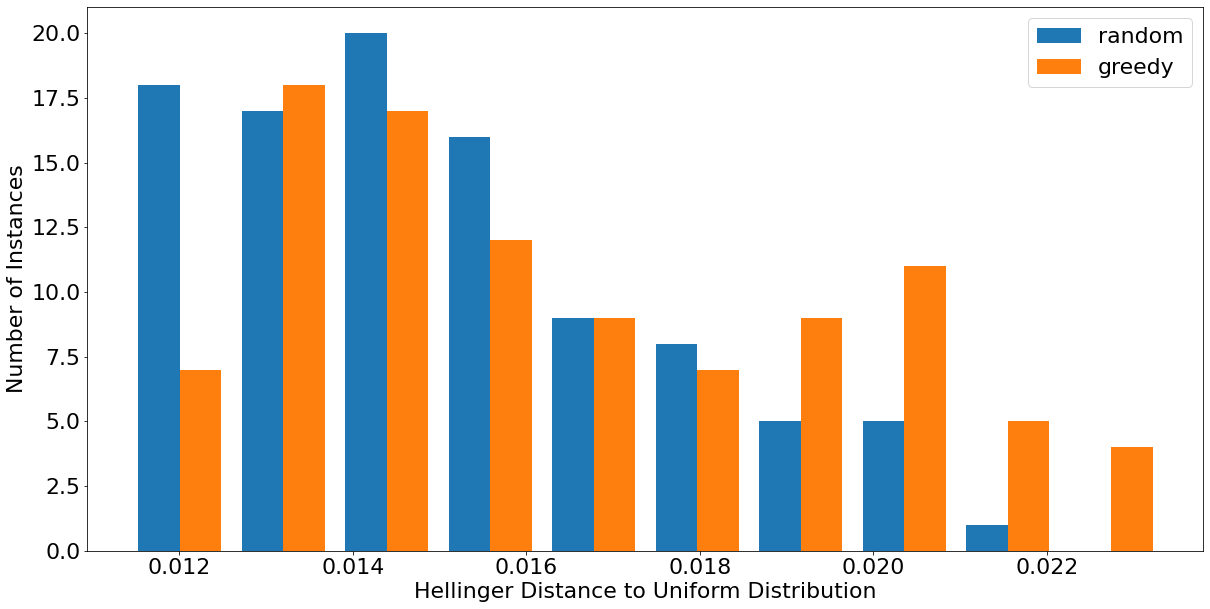
\includegraphics[width=.9\textwidth]{figures/simulations.png}
    \caption{Hellinger distance of simulated distributions to the uniform distribution using a random ordering and greedy ordering.}
    \label{Figure:simulation-results-histogram}
\end{figure}

Interestingly, the results show that the greedy ordering yields distributions that are \it{ever so slightly} less uniform than when using a random order.
This appears to contradict the conjecture we set out to gain evidence for!
However, as we noted previously, we only obtained $300$ samples out of the exponentially many possible instances of our problem.
There's nothing special about this number, we just decided to stop the simulations at a round number after several hours of computation.
The simulator scaled poorly with the number of iterations it was performing per instance.
For this reason, we were motivated to find some way to speed up the process of simulating our game.
This leads to the work done in the next section, where we completely replace the simulator with a neural network.
\subsection{Using a Neural Network}
We end up using a very simple network (\Cref{table:simple-network}) to complete our task (Other, more complex networks were experimented on and the results are compiled in \Cref{Appendix:Networks}).
We call our network \it{ARAMNet}, since our motivations came from the game of ARAM.

\begin{table}[htbp]
    \centering
    \bgroup
    \def\arraystretch{1.5}
    \begin{tabular}{|c|c|c|c|}
        \hline
        Layer       & Kernel Shape & Output Shape & \# Params \\
        \hline
        LSTM        &              & (10, 152)    & 186.048k  \\
        \hline
        BatchNorm   & (10, 1)      & (10, 152)    & 20        \\
        \hline 
        Flatten     &              & (1, 1520)    &           \\ 
        \hline
        Linear      & (1520, 1520) & (1, 1520)    & 2.31192M  \\ 
        \hline
        Reshape     &              & (10, 152)    &           \\ 
        \hline
        Softmax     &              & (10, 152)    &           \\ 
        \hline
    \end{tabular}
    \egroup
    \caption{ARAMNet}
    \label{table:simple-network}
\end{table}

The most important part we had to design into our network was the ordering of the players.
It had to be the case that if we modified the ordering, the output would reflect the change as well.
(Unless, of course, our particular instance was order-invariant)
This naturally led us to the idea of treating the $10$ players as temporal sequence of data instead of just a matrix of pool encodings.
More precisely (for those familiar with RNN-related notation), our input data is a sequence of $10$ players: $(P^{<1>}, \ldots, P^{<10>})$, which we feed into an initial layer of LSTM cells.
The network then outputs a $10$-by-$152$ matrix $M$ where $M_{ij} := \Pr(P_i \text{ selects } j)$ (i.e. The rows are precisely the discrete probability distribution for player $P_i$), performing exactly what our simulator was doing.

Although we said we would replace the simulator, we use it here one last time to generate $6000$ samples for our network to train on.
Our goal here is to minimize the Hellinger distance between the network output and simulator output, and we achieve a final training loss of $0.025$ and validation loss of $0.035$.
We train using AdamW with all the recommended settings, except for an increase in the weight decay to $0.25$, and a batch size of 16.
The learning rate was adjusted using \it{ReduceLROnPlateau}\footnote{See \url{https://pytorch.org/docs/stable/_modules/torch/optim/lr_scheduler.html\#ReduceLROnPlateau}}, a built-in Pytorch learning rate scheduler, with a patience of $4$ and a threshold of $0.01$.
The adjusting learning rate produces the bumps we see in \Cref{Figure:ARAMNet-Learning-Curve}.

\begin{figure}[htbp]
    \centering
    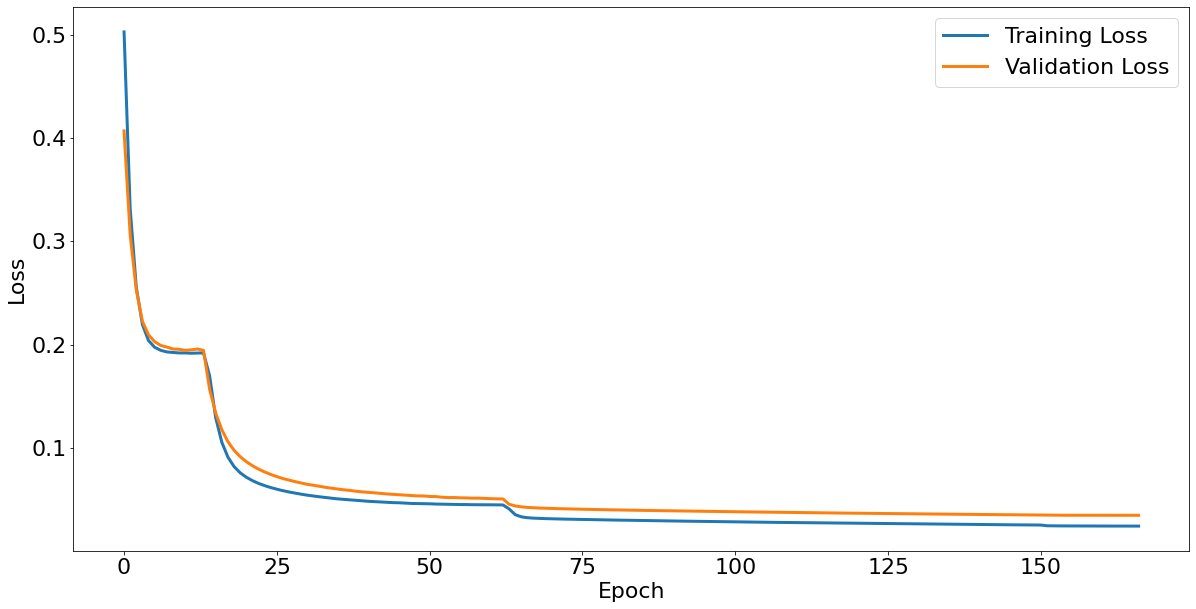
\includegraphics[width=.9\textwidth]{figures/ARAMNet-loss.png}
    \caption{Training and Validation learning curve for ARAMNet}
    \label{Figure:ARAMNet-Learning-Curve} 
\end{figure}
\subsection{Revisiting the Simulations}

Now we can revisit our simulations with a much more efficient simulation function.
This time, we simulate over $1$ million randomly generated pools, producing the results in \Cref{Figure:simulation-updated-results-histogram}.
\begin{figure}[htbp]
    \centering
    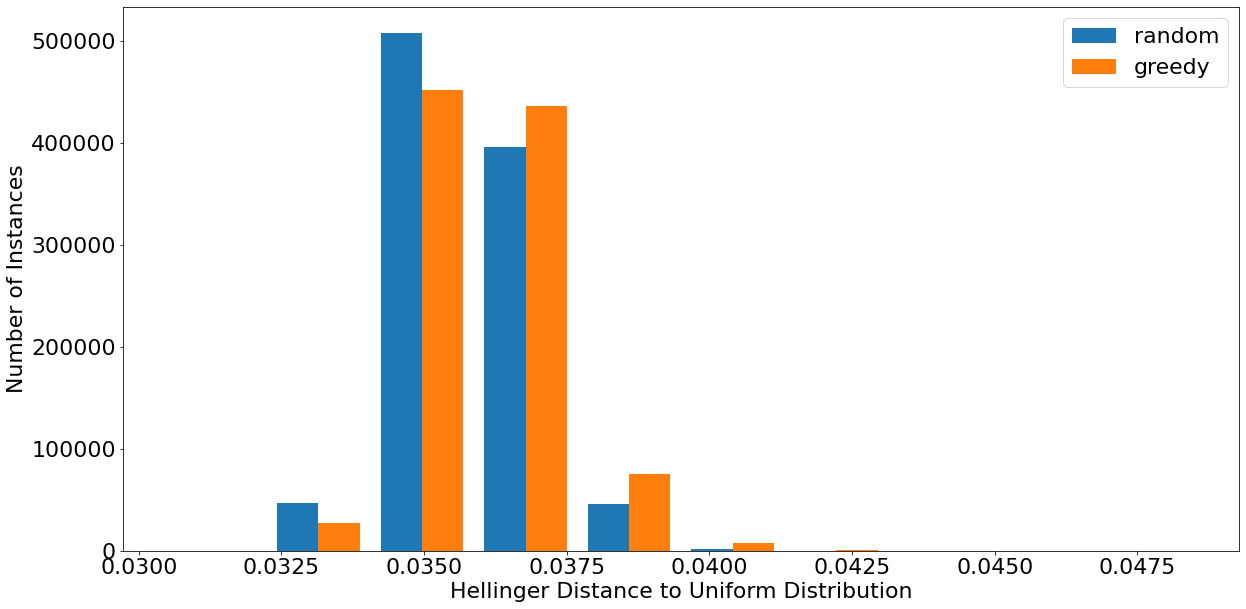
\includegraphics[width=.9\textwidth]{figures/simulations-updated.png}
    \caption{Hellinger distance of distributions produced by ARAMNet to the uniform distribution using random and greedy ordering}
    \label{Figure:simulation-updated-results-histogram}
\end{figure}
As a side remark, the reader may notice that in \Cref{Figure:simulation-updated-results-histogram} the distance to the uniform distribution is higher than in \Cref{Figure:simulation-results-histogram}.
This is expected since ARAMNet has ${\sim}0.0325$ validation loss.

\Cref{Figure:simulation-updated-results-histogram} shows that the greedy ordering produces distributions that have larger distance to the uniform distribution than when using a random ordering.
Indeed, the mean Hellinger distance to the uniform distribution is $0.03578$ when using a random ordering and $0.03603$ when using a greedy ordering.
Now, we can be a bit more sure that the phenomena we saw in \Cref{Section:Initial-Simulations} was not due to a small sample size.
In fact, it may actually be the case that the greedy ordering is not as optimal as we conjectured.
This doesn't quite disprove our conjecture since all of this evidence is empirical, but it does suggest that there may be other mechanisms at play within the player orderings.

\section{Conclusions and Outlook}\label{Section:Outlook}
We began with the very general question ``What is the best ordering for our players?''.
In completing the proof that the greedy ordering works best when there are two players, we got stuck trying to carry forward our techniques on the cases with more players.
As such, we set out to find empirical evidence that perhaps the greedy ordering is optimal for more than two players as well.
In doing so, we find that simulating this game takes an extremely long time, and as a result, created a neural network that would handle the simulations.
With that said and done, we find empirical evidence suggesting the opposite of what we set out to show: the greedy ordering is \it{not} optimal (at least for our restricted case of $152$ elements and $10$ players).
This leaves us with one last follow-up question: if the greedy ordering isn't the best ordering, what other mechanisms are at play that will determine the best ordering?

Overall, we've built some useful tools to perform empirical analysis on this problem.
In particular, the network can always be tweaked to accept different instances of our problem.
This is also the weakness of our tool as it lacks generality.
Indeed, we still lack a good grasp of the mathematics behind our problem and future research should focus on this aspect.


\clearpage
\begin{appendices}
    \section{Proof of \Cref{prop:two-player-second-case}}\label{Appendix:Proof-Of-Two-Player-Prop}

Recall the statement of our proposition: \it{If $\U_1 \setminus \U_2 \neq \emptyset$ and $|\U_1| < |\U_2|$, then $P_2$ should go first.}

Let:
\begin{itemize}
    \item $\C = \U_1 \cap \U_2 = \{c_1, \ldots, c_x\}$. We will index elements of $\C$ with $u$ (that is, $1 \leq u \leq x$ where possible)
    \item $\U_1 = \{a_1, \ldots, a_y\} \cup \C$. We will index elements of $\U_1$ with $v$ (so $1 \leq v \leq y$)
    \item $\U_2 = \{b_1, \ldots, b_z\} \cup \C$. We will index elements of $\U_2$ with $w$ (so $1 \leq w \leq z$)
\end{itemize}

By assumption, $y < z$.

\ul{$P_2$ goes first}:

\begin{equation*}
    \Pr(P_2 \text{ selects } b_w) = \Pr(P_2 \text{ selects } c_u) = \frac{1}{x + z} \quad \forall u, w
\end{equation*}

For $P_1$, we solve $\Pr(P_1 \text{ selects } a_v)$ and $\Pr(P_1 \text{ selects } c_u)$ separately:
\begin{align*}
    \Pr(P_1 \text{ selects } a_v) 
    &= \sum_w \Pr(P_1 \text{ selects } a_v \ \vert \ P_2 \text{ selects } b_w)\Pr(P_2 \text{ selects } b_w) \\
    &\quad +\sum_u \Pr(P_1 \text{ selects } a_v \ \vert \ P_2 \text{ selects } c_u)\Pr(P_2 \text{ selects } c_u) \\
    &= \sum_w \frac{1}{(x+y)(x+z)} + \sum_u \frac{1}{(x+y-1)(x+z)} \\
    &= \frac{z}{(x+y)(x+z)} + \frac{x}{(x+y-1)(x+z)} \quad \forall v
\end{align*}
\begin{align*}
    \Pr(P_1 \text{ selects } c_u) 
    &= \sum_w \Pr(P_1 \text{ selects } c_u \ \vert \ P_2 \text{ selects } b_w)\Pr(P_2 \text{ selects } b_w) \\
    &\quad +\sum_{k \neq u} \Pr(P_1 \text{ selects } c_u \ \vert \ P_2 \text{ selects } c_k)\Pr(P_2 \text{ selects } c_k) \\
    &= \sum_w \frac{1}{(x+y)(x+z)} + \sum_{k \neq u} \frac{1}{(x+y-1)(x+z)} \\
    &= \frac{z}{(x+y)(x+z)} + \frac{x-1}{(x+y-1)(x+z)} \quad \forall u
\end{align*}
Similarly, when \ul{$P_1$ goes first}:
\begin{align*}
    \Pr(P_1 \text{ selects } a_v) &= \Pr(P_1 \text{ selects } c_u) = \frac{1}{x + y} \quad \forall v, w \\
    \Pr(P_2 \text{ selects } b_w) &= \frac{y}{(x+y)(x+z)} + \frac{x}{(x+y)(x+z-1)} \quad \forall w \\
    \Pr(P_2 \text{ selects } c_u) &= \frac{y}{(x+y)(x+z)} + \frac{x-1}{(x+y)(x+z-1)} \quad \forall u
\end{align*}
In both cases, the player that goes first is granted a uniform distribution over their choices.
So, only the distribution of the 2nd player diverges from uniform.
We show that when $P_2$ goes first, the distance between the induced distribution for $P_1$ is closer to uniform than $P_2$'s induced distribution when $P_1$ goes first.

The Hellinger distance between $P_1$'s induced distribution (when $P_2$ goes first) and the uniform distribution is:
\begin{multline*}
    \sum_v \left(\sqrt{\frac{1}{x+y}} - \sqrt{\frac{z}{(x+y)(x+z)} + \frac{x}{(x+y-1)(x+z)}}\right)^2 \\ 
    + \sum_u \left(\sqrt{\frac{1}{x+y}} - \sqrt{\frac{z}{(x+y)(x+z)} + \frac{x-1}{(x+y-1)(x+z)}}\right)^2
\end{multline*}
A similar monstrosity can be produced for $P_2$'s induced distribution (when $P_1$ goes first).
The proof completes by showing the difference between the two is less than $0$ which is a routine exercise of applying the assumption that $y < z$ (the inequality $\frac{1}{(z-1)y} < \frac{1}{z(y-1)}$, which is a direct consequence of $y < z$ will also be handy) repeatedly.

    \clearpage
    \section{An Exploration into Various Neural Architectures for the Simulator Replacement}\label{Appendix:Networks}

Recall that ARAMNet (\Cref{table:simple-network}) is a very simple network consisting of a single layer of LSTM cells followed by a single linear layer.
As such, most of our exploration will be focussed on various deep versions of this.

We start with two natural deep versions of ARAMNet.
Network 2 (\Cref{Table:Network-2}) extends the number of LSTM layers, while Network 3 (\Cref{Table:Network-3}) extends the number of Linear layers.
Next, we treat ARAMNet as its own module (without the final softmax layer).
Stacking ARAMNet modules one after another gives us Network 4 (\Cref{Figure:Network-4}).
Finally, we out something really funky.
Taking inspiration by the law of total probability, we wanted to help the neural network learn that type of formula.
As such Network 5 (\Cref{Figure:Network-5}) does exactly this and perform additions and multiplications on the outputs of ARAMNet modules. 

\begin{table}[htbp]
    \centering\small
    \begin{minipage}{.49\textwidth}
        \centering
        \begin{tabular}{|c|c|c|c|}
            \hline
            Layer            & \makecell{Kernel \\ Shape} & \makecell{ Output \\ Shape} & \# Params \\
            \hline
            \makecell{LSTM \\ (3 layers)}  &              & (10, 152)    & ${\sim}558$k  \\
            \hline 
            Flatten          &              & (1, 1520)    &           \\ 
            \hline
            Linear           & (1520, 1520) & (1, 1520)    & ${\sim}2$M  \\ 
            \hline
            Reshape          &              & (10, 152)    &           \\ 
            \hline
            Softmax          &              & (10, 152)    &           \\ 
            \hline
        \end{tabular}
        \caption{Network 2 Architecture (We omit the BatchNorm layer and Dropout layers between the individual LSTM layers)}
        \label{Table:Network-2}
    \end{minipage}\hfill
    \begin{minipage}{.49\textwidth}
        \centering
        \begin{tabular}{|c|c|c|c|}
            \hline
            Layer             & \makecell{Kernel \\ Shape} & \makecell{Output \\ Shape} & \# Params   \\
            \hline
            LSTM              &              & (10, 152)    & ${\sim}184$k    \\
            \hline 
            Flatten           &              & (1, 1520)    &             \\ 
            \hline
            {\footnotesize \makecell{Linear \\ (3 Layers)}} & (1520, 1520) & (1, 1520)    & ${\sim}7$M  \\ 
            \hline
            Reshape           &              & (10, 152)    &             \\ 
            \hline
            Softmax           &              & (10, 152)    &             \\ 
            \hline
        \end{tabular}
        \caption{Network 3 Architecture (We omit the BatchNorm, Dropout and Activation layers between each Linear layer)}
        \label{Table:Network-3}
    \end{minipage}
\end{table}

\begin{figure}[htbp]
    \centering\small
    \begin{tikzpicture}
        \node[shape=rectangle, draw, thick] (1) at (0, 0) {ARAMNet};
        \node[shape=rectangle, draw, thick] (2) at (3, 0) {ARAMNet};
        \node[shape=rectangle, draw, thick] (3) at (6, 0) {ARAMNet};
        \node[vertex] (s) at (9, 0) {Softmax};
        \node[vertex] (out) at (11, 0) {$\hat{y}$};

        \draw[edge] (1) to (2);
        \draw[edge] (2) to (3);
        \draw[edge] (3) to (s);
        \draw[edge] (s) to (out);
    \end{tikzpicture}
    \caption{Network 4 Architecture Diagram}
    \label{Figure:Network-4}
\end{figure}

\begin{figure}[htbp]
    \centering\small
    \begin{tikzpicture}[scale=0.5]
        \node[shape=rectangle, draw, thick] (1) at (0, 0) {ARAMNet};
        \node[shape=rectangle, draw, thick] (2) at (0, -4) {ARAMNet};
        \node[shape=rectangle, draw, thick] (3) at (0, -8) {ARAMNet};
        \node[shape=rectangle, draw, thick] (4) at (12, -6) {ARAMNet};
        \node[vertex] (+) at (3, -2) {$+$};
        \node[vertex] (*) at (6, -6) {$*$};
        \node[vertex] (s) at (17, -6) {Softmax};
        \node[vertex] (out) at (20, -6) {$\hat{y}$};

        \draw[edge, to path={-| (\tikztotarget)}] (1) to (+);
        \draw[edge, to path={-| (\tikztotarget)}] (2) to (+);
        \draw[edge, to path={-| (\tikztotarget)}] (+) to (*);
        \draw[edge, to path={-| (\tikztotarget)}] (3) to (*);
        \draw[edge] (*) to (4);
        \draw[edge] (4) to (s);
        \draw[edge] (s) to (out);
    \end{tikzpicture}
    \caption{Network 5 Architecture Diagram}
    \label{Figure:Network-5}
\end{figure}

We trained the 4 networks on our small validation dataset of $300$ randomly generated samples, using the default settings for Adam and a batch size of 32, and plotted their learning curves alongside ARAMNet in \Cref{Figure:Training-Loss-All-Networks}.
Network 2 and (intriguingly) Network 5 were also considered as candidates to replace the simulator function.
In particular, we were very surprised that Network 5 achieved a loss matching ARAMNet.
It is, in fact, learning something interesting about the data and not just memorizing it, since the network contains ${\sim}9$ million parameters, yet, Network 3 with ${\sim}7$M performs \it{much} worse.

\begin{figure}[htbp]
    \centering
    \begin{minipage}{\textwidth}
        \centering
        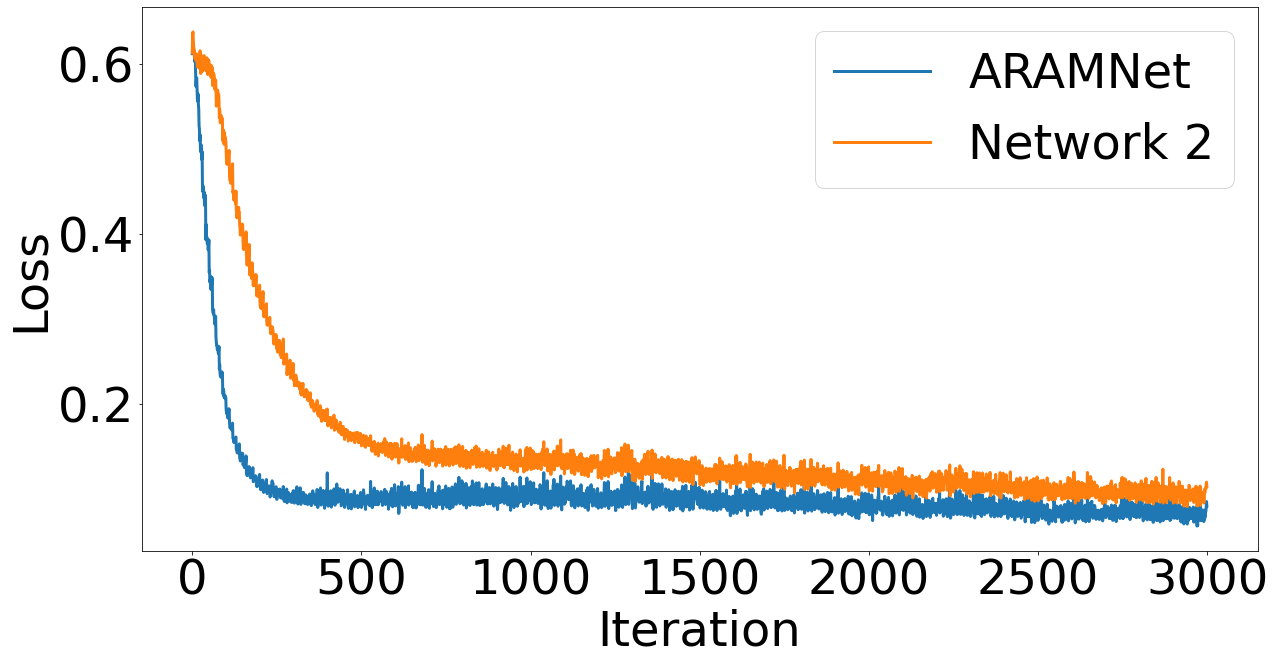
\includegraphics[width=.49\textwidth]{figures/explore-val-loss/network-2.png}\hfill
        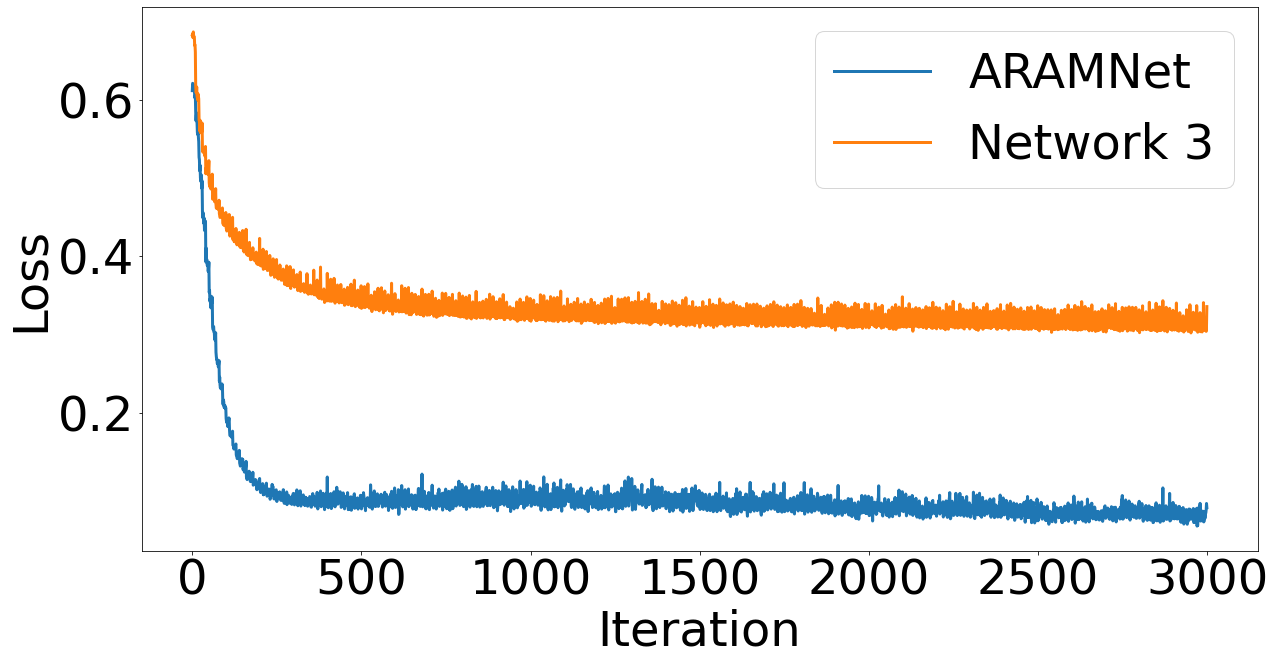
\includegraphics[width=.49\textwidth]{figures/explore-val-loss/network-3.png}
    \end{minipage}\hfill
    \vspace{3mm}
    \begin{minipage}{\textwidth}
        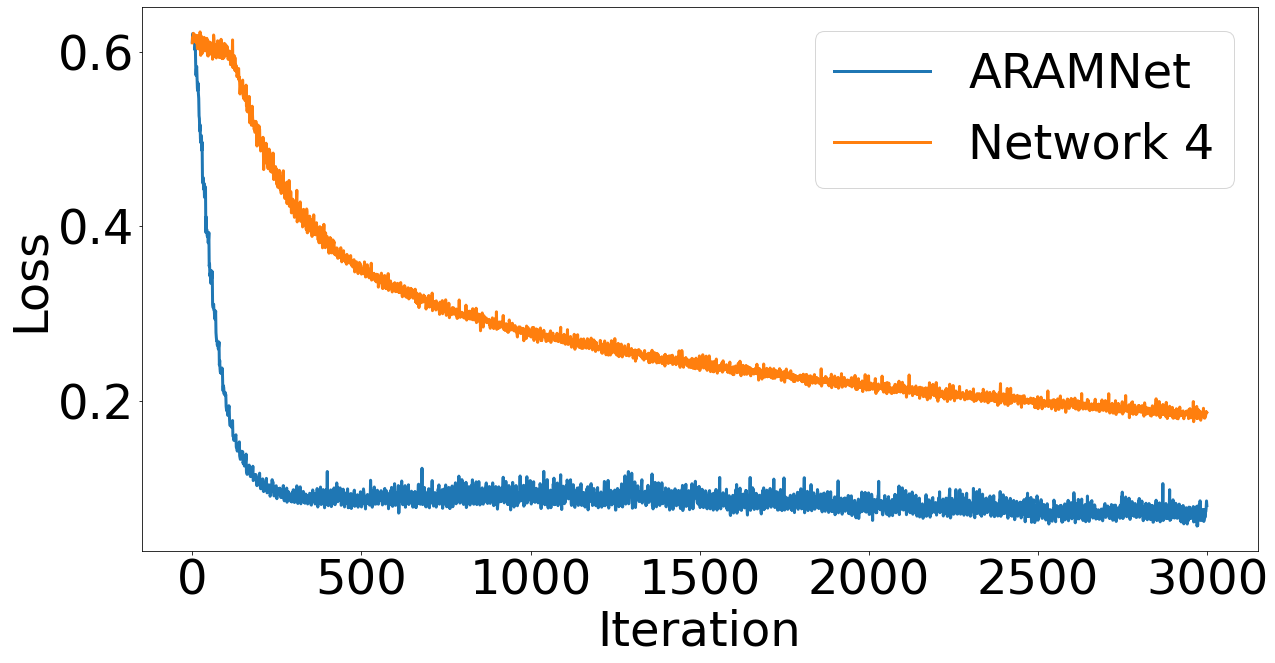
\includegraphics[width=.49\textwidth]{figures/explore-val-loss/network-4.png}\hfill
        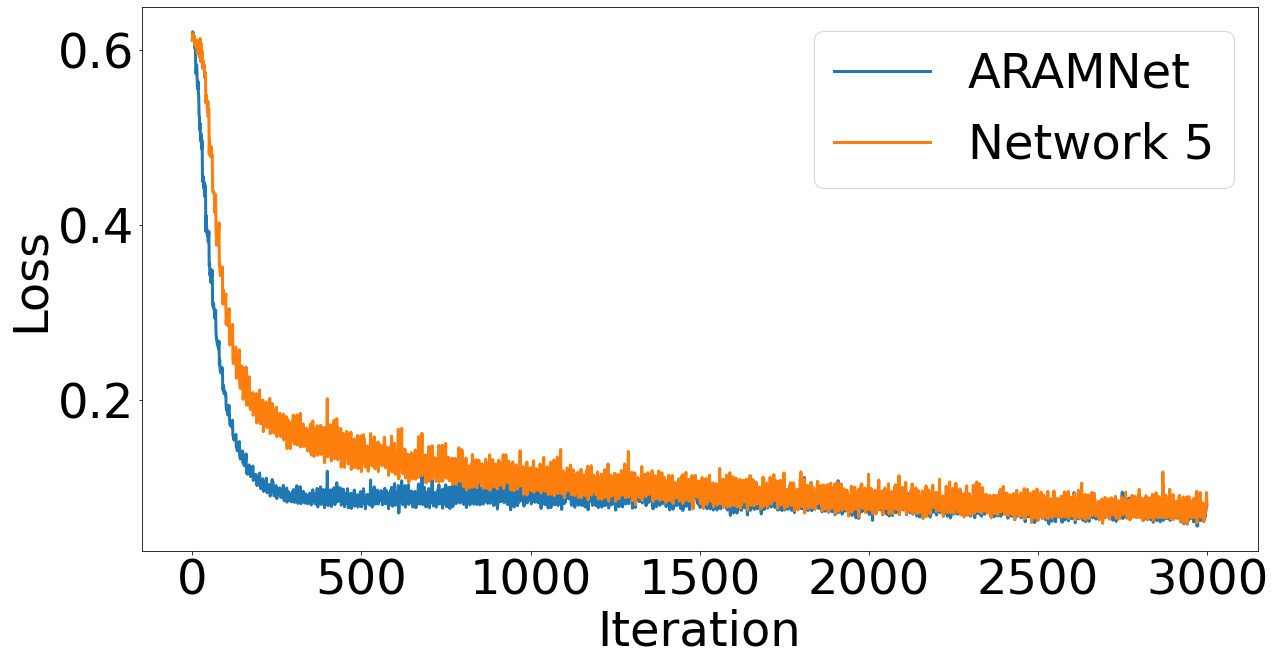
\includegraphics[width=.49\textwidth]{figures/explore-val-loss/network-5.png}
    \end{minipage}
    \caption{Learning Curve of the 4 alternate networks compared to the learning curve of ARAMNet on the validation dataset}
    \label{Figure:Training-Loss-All-Networks}
\end{figure}

However, these two networks were more difficult to train and we had trouble preventing them from overfitting.
Although they could reach training losses matching that of ARAMNet, their validation loss were much too high for them to be useful simulator replacement candidates.
In \Cref{Figure:Training-Loss-2-and-5}, we can see just how large the training-to-validation loss gap is, as compared to \Cref{Figure:ARAMNet-Learning-Curve}.

\begin{figure}
    \centering
    \begin{minipage}{\textwidth}      
        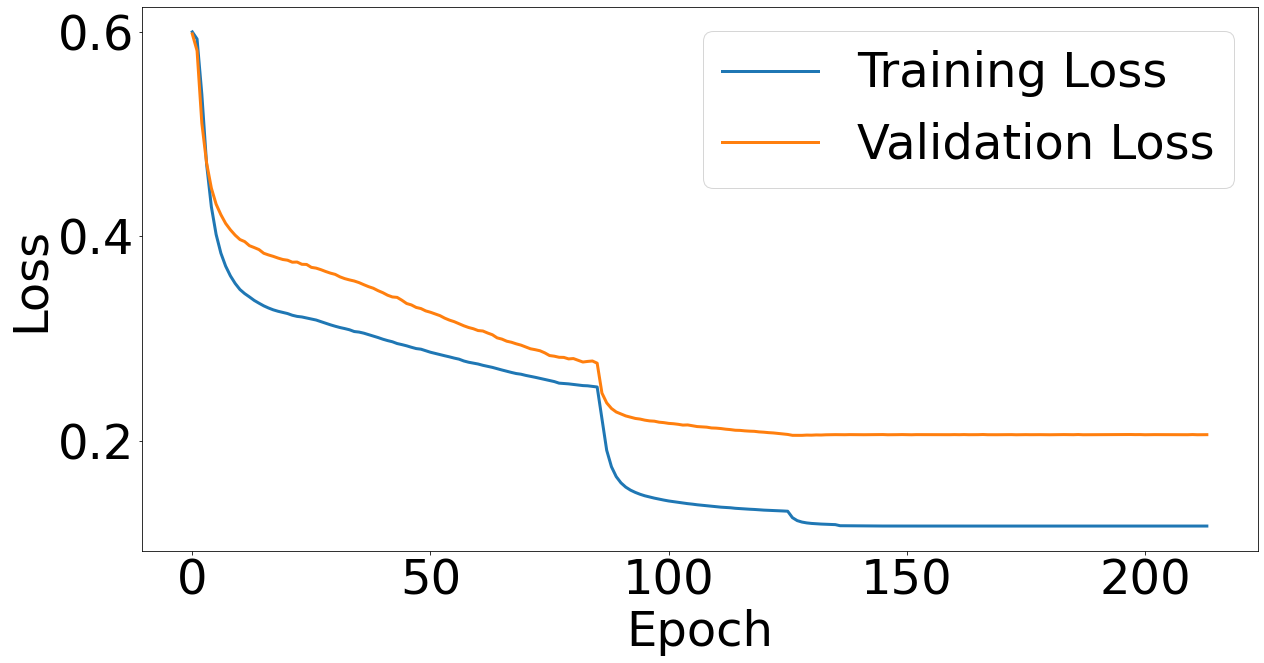
\includegraphics[width=.49\textwidth]{figures/explore-train-loss/network-2.png}\hfill
        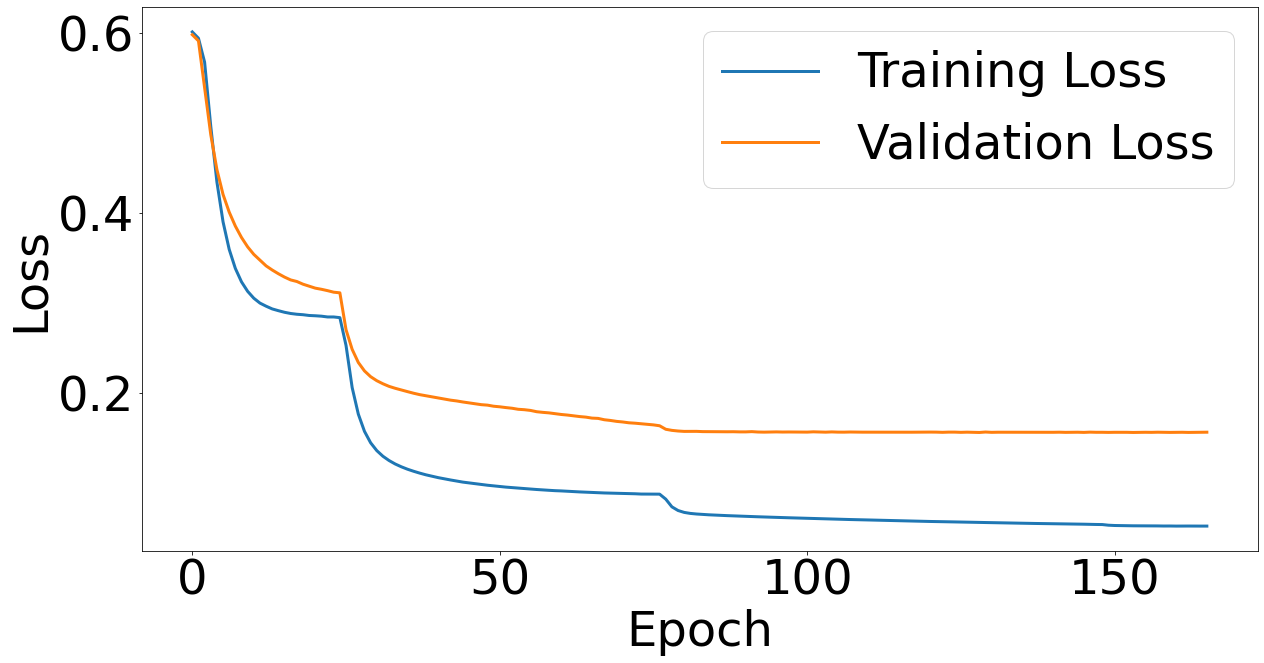
\includegraphics[width=.49\textwidth]{figures/explore-train-loss/network-5.png}
    \end{minipage}
    \caption{Learning curves for Networks 2 and 5 when we trained using the same optimizer and settings as with ARAMNet.}
    \label{Figure:Training-Loss-2-and-5}
\end{figure}
\end{appendices}


\end{document}